


\noindent {\color{special}{\Large \bf LIÇÃO 1 - Para o professor}}
\vspace{.5cm}

Esta lição tem por objetivo introduzir frações unitárias a partir de modelos contínuos, tais como círculos, retângulos, hexágonos e segmentos, fazendo uso de expressões verbais como, por exemplo, metade de, um terço de, a terça parte de, um quarto de, para indicar essas frações.
Uma vez estabelecida a unidade, a expressão ``fração unitária'' nomeia cada uma das partes da divisão da unidade em partes iguais.

As atividades visam à equipartição de uma unidade. Equipartição entendida como partição em partes iguais, sem que as partes tenham necessariamente a mesma forma. Assim, por exemplo, na equipartição de um retângulo está implícito que as partes têm a mesma área, e não necessariamente a mesma forma nem o mesmo perímetro. O objetivo é levar o aluno a reconhecer diferentes modos de dividir e recompor a unidade. No senso comum, as expressões repartir, partir e dividir são sinônimas e não pressupõem a equipartição. No entanto, é importante lembrar que, no caso da operação de divisão, espera-se que o resultado registre uma equipartição. No futuro, o estudante deverá entender um terço como o resultado da divisão de um por três. Este é o caso da operação, em que a palavra ``divisão'' abrevia ``divisão em partes iguais''.

Espera-se que, ao final da lição, os alunos saibam identificar e representar frações unitárias a partir de modelos  diversos, fazendo o uso adequado de expressões verbais para nomeá-las. No entanto, o professor não deve apresentar o termo ``fração unitária'' ao estudante, uma vez que é desnecessário para a aprendizagem pretendida. Fazê-lo pode, inclusive, comprometer o que se pretende com a lição. Não se pretende apresentar aos alunos a linguagem simbólica de frações, que será tratada nos capítulos seguintes.

De maneira geral, as atividades envolvem a abordagem das frações unitárias com objetivos diversos. Por exemplo, diferenciar a divisão da unidade em partes ``quaisquer'' da divisão da unidade em partes ``iguais'' (equipartição); reconhecer a necessidade de uma expressão verbal que identifique uma das partes iguais em uma equipartição da unidade; perceber que a unidade pode ser subdividida em uma quantidade igual de partes sem que essa divisão represente uma equipartição; reconhecer que em modelos contínuos, as partes de uma equipartição podem não ter a mesma forma; distinguir uma equipartição específica dentre partições diversas ou reconhecer a quarta parte como a metade da metade.

A participação do aluno, criando representações próprias e fazendo uso da linguagem verbal para explicar o seu raciocínio diante da realização das atividades, será fundamental na condução desta seção.
\vspace{.15cm}

\noindent OBJETIVOS ESPECÍFICOS DA LIÇÃO 1:
\vspace{.15cm}

\noindent O aluno deve ser capaz de:
\begin{itemize}
\item  Diferenciar uma partição qualquer de uma unidade de uma equipartição (partição em partes iguais) de uma mesma unidade.
\item Reconhecer a necessidade de uma expressão verbal que identifique uma das partes iguais em uma equipartição da unidade.
\item  Reconhecer que em modelos contínuos, as partes de uma equipartição podem não ter a mesma forma.
\item  Identificar, a partir de representações visuais diversas, frações unitárias de denominador variando de 2 a 10.
\item  Utilizar a linguagem verbal que caracteriza as frações unitárias de denominador variando de 2 a 10. (Isto é, ``metade de'', ``um meio'', ``um terço'', ``terça parte de'', ..., ``um décimo'', ``décima parte de'').
\item  Comparar frações unitárias em exemplos concretos simples (por exemplo, reconhecer que um terço de uma pizza é maior do que um quarto da mesma pizza).
\item  Recompor a unidade a partir de uma fração unitária dada em modelos contínuos.
\item  Relacionar uma fração da unidade à quantidade necessária dessas partes para compor a unidade. Assim, por exemplo, é necessário reunir cinco {\textit quintas partes} para recompor a unidade.
\end{itemize}

\begin{multicols}{2}

%{Atividade 1}  
\begin{objetivos}{}{}
\begin{itemize} %s
    \item       Diferenciar a partição da unidade em partes ``quaisquer'' da partição da unidade em partes       ``iguais''. 
    \item       Reconhecer a necessidade de uma expressão verbal que identifique uma das partes iguais em uma equipartição da unidade.
    \item       Diferenciar ``a partição da unidade em três partes quaisquer'' da ``partição da unidade em três partes iguais''.
    \item       Compreender as expressões ``um terço de'' e ``terça parte de'' como formas de identificar uma das partes da equipartição da unidade em três partes.
\end{itemize} %s
\end{objetivos}

\begin{orientacoes}
  \begin{itemize} %s
  \item No final deste volume estão disponíveis materiais para reprodução. Mas o professor pode usar folhas de papel para o mesmo fim.
  \item Recomenda-se que a atividade seja desenvolvida em grupos de 3 a 5 alunos.
  \item A partição em partes iguais será chamada neste texto de ``equipartição'', mas consideramos desnecessário o uso desta palavra pelo professor com os estudantes. O objetivo é fazer a equipartição livremente de forma coerente. Assim, por exemplo, podem ser aceitas como respostas:
    \begin{center}
      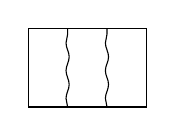
\begin{tikzpicture}[scale=.5]
   \draw (0,0) rectangle (3,2);
   \draw[decorate, decoration={snake, amplitude= .2 mm}] (1,0) -- (1,2);
   \draw[decorate, decoration={snake, amplitude= .2 mm}] (2,0) -- (2,2);        
      \end{tikzpicture}
    \end{center}
  \item  Não se espera que, nesta atividade, os alunos usem a medida para fazer a equipartição de maneira precisa.
    \item Busque conduzir a discussão nos grupos de modo que os estudantes percebam que, para que os amigos recebam a mesma quantidade de chocolate, a partição proposta para a barra de chocolate deve ser em ``partes iguais'', no sentido de ganharem todos a mesma quantidade de chocolate, não necessariamente pedaços de mesma forma.
    \item Na discussão, procure destacar que a referência à ``partição em três partes iguais'' se dá a partir das expressões ``um terço'' da barra de chocolate ou ``a terça parte'' da barra de chocolate.
    \item O item c) admite diversas soluções, algumas estão apresentadas como resposta. No entanto, algumas dessas respostas podem não aparecer naturalmente em sala de aula. Avalie a possibilidade de apresentar e explorar algumas dessas soluções (ou outras que queira) em sala de aula. Por exemplo, apresente uma dessas divisões aos alunos e peça-lhes que avaliem a equipartição, explicando sua decisão.
    \item O item d), provavelmente, pode não ser respondido corretamente pelos alunos. Se for o caso, as expressões ``um terço de'' e ``a terça parte de'' devem ser apresentadas.
    \item Fique atento às falas dos alunos. Observe que os alunos podem representar e verbalizar as respostas de diferentes modos e que não há uma resposta única para a atividade. Por exemplo, alguns alunos podem precisar de mais tempo do que outros para usar a expressão       ``um terço'' no lugar de       ``partição em três partes iguais'' ou ``divisão em três partes iguais''. Ou ainda, observarem que há diferentes representações para a equipartição.
      \item Pode ser aproveitada a oportunidade para questionar os estudantes se no lugar de três amigos fossem 5 amigos, cada um receberia mais ou menos chocolate após a divisão em cinco partes iguais? 
\end{itemize} %s


\begin{itemize} %s
    \item Esta atividade pode ser adaptada visando a inclusão de alunos com deficiência de visão. Para isso, sugere-se confeccionar os modelos da barra de chocolate  inteira e repartida, que estão disponíveis para reprodução no final do livro, em três materiais diferentes. Por exemplo, papel comum e papéis com texturas diferentes, tecido ou material emborrachado.
\end{itemize} %s
\end{orientacoes}
%\vfill
\begin{solucao}{}{}
  \begin{enumerate}[a),wide,labelindent=0pt] %s
    \item       Este item não possui resposta correta, apenas respostas coerentes com a explicação do aluno. Por exemplo, um estudante pode dizer que sim e explicar que o amigo mais velho deve ficar com uma parte maior porque precisa de mais energia. Mas a resposta esperada é que a divisão não parece justa porque as quantidades de chocolate são diferentes. Discuta com os alunos para que entendam a divisão correspondente à resposta esperada.
    \item Não, eles receberão quantidades diferentes de chocolate, embora cada um receba um único pedaço do chocolate.
    \item Respostas possíveis:

  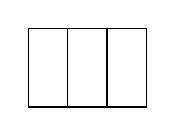
\begin{tikzpicture}[scale=.5]
   \draw (0,0) rectangle (3,2);
   \draw (1,0) -- (1,2);
   \draw (2,0) -- (2,2);
  \end{tikzpicture}
  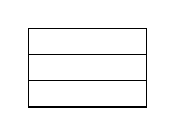
\begin{tikzpicture}[scale=.5]
   \draw (0,0) rectangle (3,2);
   \draw (0,.6666) -- (3,.6666);
   \draw (0,1.3333) -- (3,1.3333);
  \end{tikzpicture}
  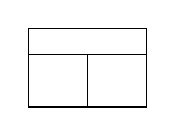
\begin{tikzpicture}[scale=.5]
   \draw (0,0) rectangle (3,2);
   \draw (0,1.3333) -- (3,1.3333);
   \draw (1.5,0) -- (1.5,1.333);
  \end{tikzpicture}
  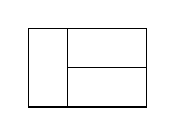
\begin{tikzpicture}[scale=.5]
   \draw (0,0) rectangle (3,2);
   \draw (1,0) -- (1,2);
   \draw (1,1) -- (3,1);
  \end{tikzpicture}

  %\noindent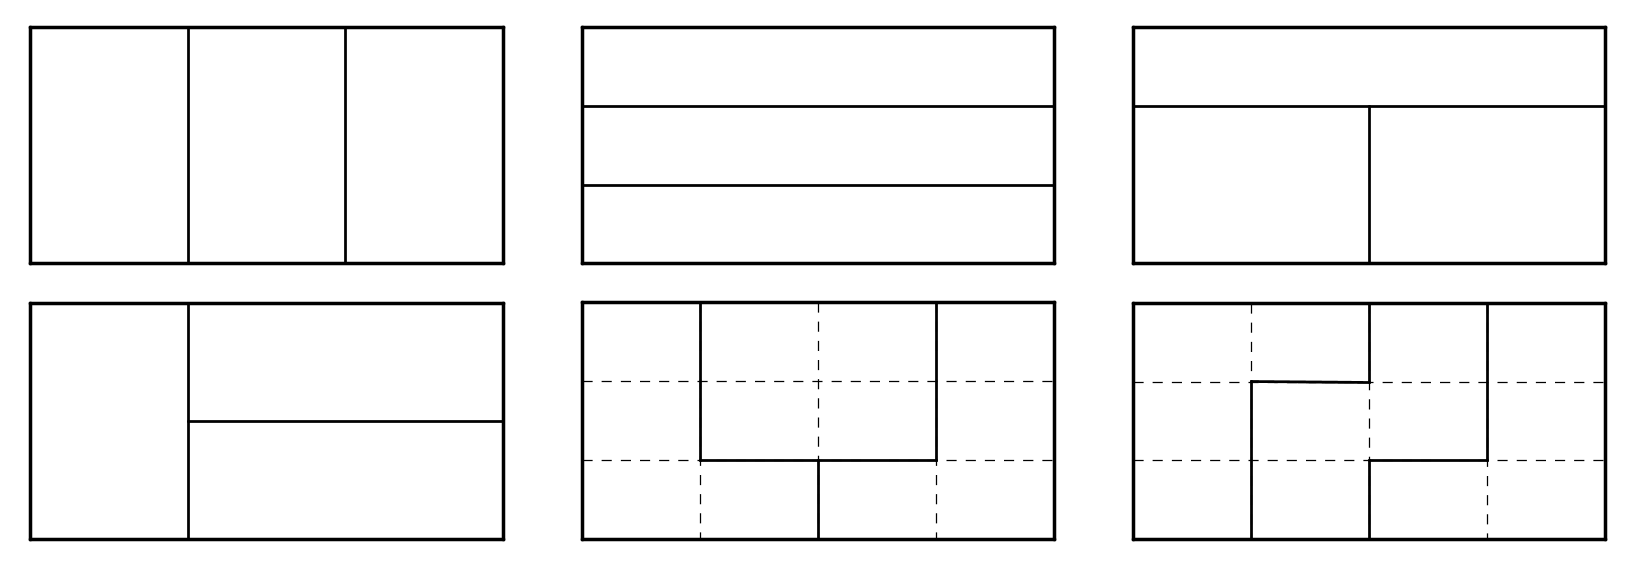
\includegraphics[width=.45\textwidth, keepaspectratio]{../..//media/cap1/secoes/licao1_atv1.png}
    \item       Cada parte é {\it um terço} da barra ou a {\it terça parte} da barra.
\end{enumerate} %s
\end{solucao}

%\subsection{Atividade 2}

\begin{objetivos}{}{}
\begin{itemize} %s
    \item       Perceber que uma unidade (no caso, uma pizza) pode ser subdividida em um mesmo número de partes sem que cada divisão represente uma equipartição.
    \item       Distinguir uma equipartição dentre partições diversas.
    \item       Diferenciar       ``a divisão da unidade em quatro partes quaisquer'' da       ``divisão da unidade em quatro partes iguais''.
    \item       Compreender as expressões ``um quarto de'' e ``quarta parte de'' como forma de identificar uma das partes da equipartição em 4 partes.
\end{itemize} %s
\end{objetivos}

\begin{orientacoes}
  \begin{itemize} %s
    \item No final deste volume estão disponíveis materiais para reprodução.
    \item Recomenda-se que a atividade seja desenvolvida em grupos de 3 a 5 alunos.
    \item As diversas soluções apresentadas pelos diferentes grupos devem ser discutidas com a turma inteira.
    \item É importante que a discussão conduza os alunos ao entendimento de que apenas as partes da equipartição podem ser chamadas de ``quartos'' da pizza, as demais são simplesmente fatias ou pedaços, por exemplo.
    \item Os alunos devem reconhecer que, apesar de todas as pizzas estarem repartidas em quatro fatias, apenas uma das repartições propostas sugere a equipartição, respondendo assim a último item desta atividade.
    \item       Essa atividade pode ser adaptada visando à inclusão de alunos com deficiência visual. Para isso, sugere-se confeccionar os modelos das três pizzas repartidas, que estão disponíveis para reprodução no final do livro, em três materiais diferentes. Por exemplo, papel comum e papéis com texturas diferentes, tecido ou material emborrachado.
\end{itemize} %s
\end{orientacoes}

\begin{solucao}{}{}
\begin{enumerate} [a),wide,labelindent=0pt] %d
    \item       Sim. Cada grupo repartiu sua pizza em quatro fatias.
    \item       Não, pois algumas fatias têm quantidades de pizza diferentes das outras.
    \item       Apenas no grupo 1 as 4 crianças receberam a mesma quantidade de pizza. Cada fatia da pizza do grupo 1 é {\it um quarto} da pizza ou {\it a quarta parte} da pizza.
\end{enumerate} %d
\end{solucao}



\begin{objetivos}{}{}
\begin{itemize} %s
    \item       Reconhecer a equipartição em um modelo linear.
    \item       Reconhecer a quarta parte como a metade da metade.
\end{itemize} %s
\end{objetivos}

\begin{orientacoes}
\begin{itemize} %s
   \item No final deste volume estão disponíveis materiais para reprodução. Esta atividade necessita deste material.
   \item Recomenda-se que esta atividade seja desenvolvida em grupos de quatro alunos.
   \item       Cada grupo deve receber um pedaço de barbante de, aproximadamente, 1m e quatro enfeites (todos iguais).
    \item       Os quatro enfeites precisam ser confeccionados antes da realização da tarefa. Sugerem-se estrelas, cujos modelos estão disponíveis para reprodução no final do livro. No entanto, segundo a avaliação do professor, os enfeites podem ser outros, desde que sejam os 4 congruentes.
    \item       Como sugestão, se possível, solicitar aos alunos que confeccionem os enfeites, por exemplo, associando esta atividade com geometria, com a abordagem de grandezas e medidas, com a disciplina de artes ou envolvendo culturas artesanais populares.
    \item       A equipartição do barbante não deve ser obtida a partir da medida do barbante, mas por sucessivas dobras do barbante sobre ele mesmo, como ilustrado na resposta da atividade. Tal discussão também  será útil na abordagem de frações equivalentes na Lição 4.
    \item       A manipulação e a dobra do barbante devem sustentar a discussão para a identificação da       ``metade da metade'' com a       ``quarta parte'' do barbante. Nesse caso, a identificação se dará pela sobreposição das partes.
      \item Nossa experiência aplicando esta atividade tem mostrado um efeito emocional positivo em permitir que os estudantes realmente confeccionem os enfeites.
\end{itemize} %s

%\vspace*{\fill}
%\columnbreak
\end{orientacoes}

\begin{solucao}{}{}
Uma maneira de se cortar o barbante é dobrar ao meio e depois dobrar novamente ao meio, obtendo quatro partes iguais, como ilustrado na figura a seguir.
  \begin{center}
  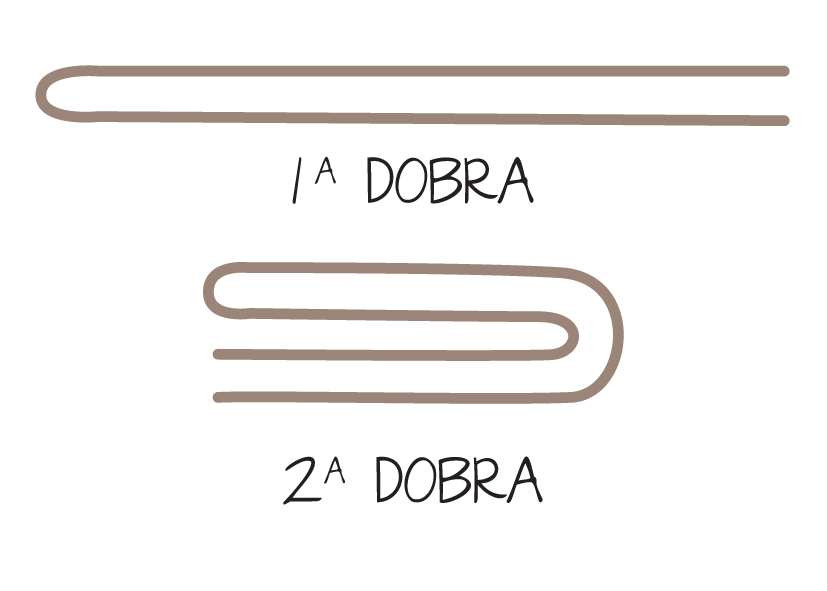
\includegraphics[width=200pt, keepaspectratio]{../figuras/licao01/ativ3_fig03.png}
  \end{center}
\end{solucao}
\end{multicols}

\subsection{Sobre o Organizando as Ideias}

  Nesta etapa, espera-se que os alunos compreendam as frações como forma de expressar quantidades. O objetivo é que percebam seu papel para expressar quantidades em situações de equipartição da unidade. Assim, as frações podem ser utilizadas no dia a dia para identificar quantidades do mesmo modo que os números naturais, já conhecidos dos alunos. Por exemplo, como nas expressões:   ``dois ovos'',   ``duas xícaras de farinha'',   ``um terço de xícara de cacau'' e   ``meio litro de leite''.

  Objetiva-se a expressão verbal e não a representação simbólica. Espera-se, assim, que os alunos apropriem-se das expressões verbais que identificam as frações unitárias (um meio, um terço, um quarto, ... , um nono e um décimo) antes de serem apresentados formalmente à simbologia matemática (que será objetivo da próxima lição).  A referência às frações unitárias com a expressão   ``um'' antes da identificação da parte, como, por exemplo, em   ``um terço'' e em   ``um sétimo'', é uma decisão pedagógica. Claro que é possível referir-se a essas frações simplesmente por   ``terço'' e   ``sétimo'', respectivamente. No entanto, nas próximas seções, pretende-se que as frações não unitárias, como   ``dois terços'' e ``nove sétimos'', por exemplo, sejam entendidas a partir da justaposição das frações unitárias correspondentes, o que é naturalmente amparado pela contagem. Nas expressões verbais relativas às frações unitárias, o   ``um'' antes da identificação da parte está associado à contagem. Dessa forma, a compreensão das frações   ``um terço'' e   ``dois terços'' ou das frações ``um sétimo'' e ``nove sétimos'', por exemplo, seguem a mesma construção lógica.

\Bg

\begin{multicols}{2}
\begin{objetivos}{}{}
  \begin{itemize} %s
    \item       Reconhecer que, em uma equipartição, as partes podem não ter a mesma forma.
    \item       Identificar a equivalência entre as partes de uma equipartição a partir de sobreposição ou da comparação pelo reconhecimento da associação a uma mesma fração unitária (no caso,um quarto).
    \item       Reconhecer a quarta parte como a metade da metade.
\end{itemize} %s
\end{objetivos}

\begin{orientacoes}
  \begin{itemize} %s
    \item No final deste volume estão disponíveis materiais para reprodução. Cada estudante deve receber os oito retângulos coloridos
    \item Recomenda-se que esta atividade seja desenvolvida em grupos de 3 a 5 alunos.
    \item Caso não seja possível imprimir os retângulos em cores, use a versão em preto e branco, também disponível no final do livro, e peça para os estudantes colorirem. O objetivo das cores é facilitar a identificação dos retângulos na discussão em sala.
    \item É importante observar que todos os retângulos estão divididos em quartos. Conduza a discussão de modo a levar os alunos a reconhecer que, em uma equipartição, as partes não precisam ter a mesma forma.
    \item Nesta atividade, espera-se que os alunos consigam lidar com a figura de um retângulo como representativa de uma unidade genérica.  No entanto, se necessário, o professor pode associar cada retângulo a um objeto concreto (por exemplo, uma barra de chocolate ou a um pedaço de bolo).
    \item É esperado que não seja imediato o reconhecimento de que as partes dos retângulos da segunda linha representam quartos. Nesse caso,  uma alternativa possível é solicitar que eles recortem as partes de cada um dos retângulos da primeira linha para realizar a comparação por sobreposição com as partes dos retângulos da segunda linha.
   \item Recomenda-se ressaltar para os estudantes ao término da atividade que um quarto é a metade da metade.
    \item Em alguns casos, a comparação se dará pela identificação da fração unitária correspondente a cada parte. Nesses casos, o aluno deve reconhecer que a quarta parte é equivalente à metade da metade. Por exemplo, como no caso seguir.
 
\end{itemize} %s

\noindent 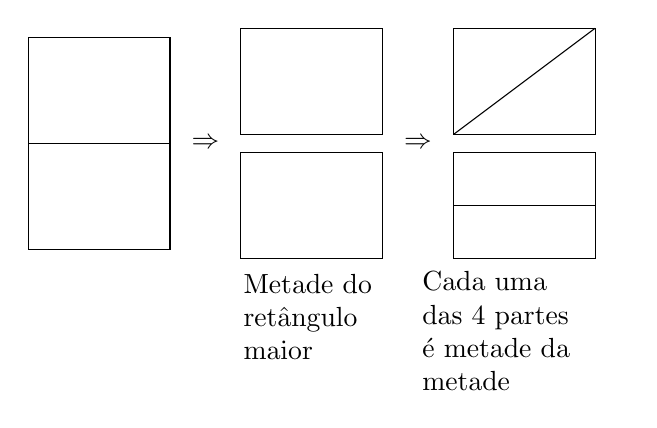
\begin{tikzpicture}[scale=0.45]
  \draw (0,0) rectangle (4,3);
  \draw (0,3) rectangle (4,6);
 % \draw (0,1.5) -- (4,1.5);
  \draw (5,3) node{$\Rightarrow$};
  \draw (6,-0.25) rectangle (10,2.75);
  \draw (6,3.25) rectangle (10,6.25);
  \node[text width=2cm]  at (8.3,-1.9) {Metade do retângulo maior};
  \draw (11,3) node{$\Rightarrow$};
  \draw (12,-0.25) rectangle (16,2.75);
  \draw (12,3.25) rectangle (16,6.25);
  \draw (12,3.25) -- (16,6.25);
  \draw (12,1.25) -- (16,1.25);
  \node[text width=2.5cm]  at (13.9,-2.3) {Cada uma das 4 partes é metade da metade};
  \end{tikzpicture}
\begin{itemize} %s
\item Segundo a avaliação do professor, a atividade pode ser realizada em duas etapas. Em um primeiro momento, os alunos recebem as primeiras quatro das oito imagens e realizam a atividade com essas imagens - cuja comparação se dá apenas pela sobreposição. Em seguida, recebem as outras quatro, para concluir a atividade. 

\item Da experiência dos autores com a implementação desta atividade em sala de aula, constatou-se uma empolgação dos estudantes quando, ao percebem que formas diferentes podem representar a mesma fração da unidade, foram convidados a gerarem outras equipartições dessa unidade. Seguem outras possíveis equipartições:

  \begin{center}
    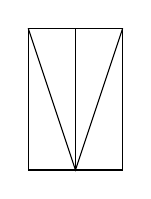
\begin{tikzpicture}[scale=.3]
      \draw[black] (0,0) rectangle (4,6);
      \draw (2,0) -- (2,6);
      \draw (0,6) -- (2,0) -- (4,6);
    \end{tikzpicture}\quad\quad\quad
        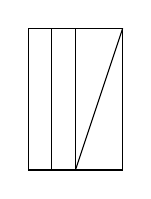
\begin{tikzpicture}[scale=.3]
      \draw[black] (0,0) rectangle (4,6);
      \draw (2,0) -- (2,6);
      \draw (1,0) -- (1,6);
      \draw (2,0) --  (4,6);
    \end{tikzpicture}\quad\quad\quad
        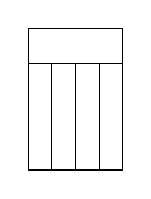
\begin{tikzpicture}[scale=.3]
      \draw[black] (0,0) rectangle (4,6);
      \draw (1,0) -- (1,4.5);
      \draw (2,0) -- (2,4.5);
      \draw (3,0) -- (3,4.5);
      \draw (0,4.5) --  (4,4.5);
    \end{tikzpicture}
  \end{center}
\end{itemize} %s
\end{orientacoes}

\begin{solucao}{}{}
\begin{enumerate}[a),wide,labelindent=0pt] %s
    \item       Todos os retângulos estão divididos em quartos.
    \item       Dois desenhos possíveis são:
\begin{center}
    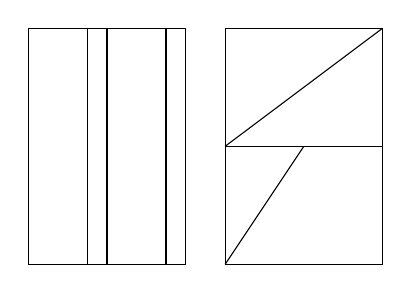
\begin{tikzpicture}[scale=5, x=1mm, y=1mm]
  \draw (0,0) rectangle (1.5,6);
  \draw (1.5,0) rectangle (2,6);
  \draw (2,0) rectangle (3.5,6);
  \draw (3.5,0) rectangle (4,6);
  \draw (5,0) rectangle (9,3);
  \draw (5,3) rectangle (9,6);
  \draw (5,0) -- (7,3);
  \draw (5,3) -- (9,6);
\end{tikzpicture}
\end{center}
\end{enumerate} %s
\end{solucao}

\clearpage
\begin{objetivos}{}{}
Relacionar uma fração unitária à unidade correspondente por recomposição. Por exemplo, reconhecer que é necessário reunir cinco quintas partes para recompor a unidade.
\end{objetivos}

\begin{orientacoes}
  
\end{orientacoes}

\begin{solucao}{}{}
  
\end{solucao}

\end{multicols}

\newpage
\begin{objetivos}{}{}
\begin{itemize} %s
    \item       Identificar uma mesma fração unitária (no caso, a terça parte) em representações diversas.
\end{itemize} %s
\end{objetivos}

\begin{orientacoes}

\begin{itemize} %s
    \item       Recomenda-se que esta atividade seja desenvolvida em grupos de 3 a 5 alunos.
    \item       Durante a discussão, os alunos devem ser estimulados a explicar as suas escolhas. A discussão sobre os motivos da identificação, ou não, de cada uma das representações à terça parte da unidade correspondente será fundamental para atingir o objetivo da atividade.
    \item       Os alunos devem reconhecer que, seja qual for a unidade considerada, em uma equipartição em 3 partes, cada uma das partes é um terço (ou a terça parte) da unidade.
    \item       Aproveite as próprias palavras e os argumentos dos alunos para conduzi-los às conclusões esperadas.
    \item       Fique atento aos alunos que selecionarem as figuras que simplesmente possuem alguma associação com o número 3, não correspondendo a terços. Por exemplo, um aluno que associe a       {\bf Figura f)} a terços pode ainda não ter compreendido a necessidade da equipartição para a identificação de um terço. Já o aluno que associa       {\bf Figura g)}       a terços pode estar simplesmente contando as partes em vermelho, sem que tenha reconhecido que a figura deveria estar dividida em 3 partes iguais e não em 5.
\end{itemize} %s
\end{orientacoes}

\begin{solucao}{}{}
A parte em vermelho representa um terço da figura nos itens b), c), e), h) e j).
\end{solucao}

\newpage

\begin{objetivos}{}{}
  \begin{itemize} %d
    \item       Recompor a unidade a partir de uma fração unitária dada em modelos contínuos.
    \item       Relacionar uma fração da unidade à quantidade necessária dessas partes para compor a unidade. Assim, por exemplo, é necessário reunir cinco       {\it quintas partes}       para recompor a unidade.
\end{itemize} %d
\end{objetivos}

\begin{orientacoes}
  \begin{itemize} %d
  \item Recomenda-se que a atividade seja desenvolvida em grupos de 3 a 5 alunos.
    \item No final deste volume estão disponíveis materiais para
reprodução para esta atividade.
    \item É importante ter em mente que existem várias soluções para cada item. Por exemplo, o primeiro item pode ser corretamente respondido por             \begin{tikzpicture}[scale=.2]
\draw [fill=common, fill opacity=.3] (0,0) arc (0:180:3) -- (0,0) -- cycle;
\draw (-3,0) -- (-3,3);
\end{tikzpicture}
 ou por
 \begin{tikzpicture}[scale=.2]
\draw [fill=common, fill opacity=.3] (0,0) arc (0:90:3) -- (-3,0) -- cycle;
\draw [fill=common, fill opacity=.3] (-3,0) arc (270:180:3) -- (-3,3) -- cycle;
\end{tikzpicture}.
\item O primeiro item pode ser corretamente respondido com
  \begin{tikzpicture}[scale=.2]
\draw [fill=common, fill opacity=.3] (0,0) arc (0:90:3) -- (-3,0) -- cycle;
\draw [fill=common, fill opacity=.3] (3.7,0) arc (0:90:3) -- (0.7,0) -- cycle;
\end{tikzpicture}
No entanto, para isso, espera-se que o estudante reconheça que essas duas partes separadas compõem uma só unidade. Sugerimos que o professor apenas discuta esse tipo de resposta, caso algum estudante a apresente. 
    \item Estimule os alunos a reconhecer (e a fazer) mais do que uma representação para a unidade em cada item.
    \item Estimule os alunos a, a partir da identificação da fração unitária, determinar a quantidade de partes necessárias para recompor a unidade.
\end{itemize} %d
\end{orientacoes}

\begin{solucao}{}{}
Algumas possibilidades de respostas:
\begin{center}

 \def \sc {0.22}
 \def\h{1.8}
 
  \begin{longtable}{|m{0.2\linewidth}|m{0.3\linewidth}|m{0.4\linewidth}|}
  \hline
\centering Fração da unidade & \centering Nome da fração da unidade  & \quad\quad\quad Unidade  \\
\hline \hline
\endhead
\centering \begin{tikzpicture}[scale=\sc]
 \draw [fill=common, fill opacity=.3] (0,0) arc (0:90:3) -- (-3,0) -- cycle;
\end{tikzpicture}
&\centering \parbox[c][\h cm][c]{0.01cm}{  } metade  & \begin{tikzpicture}[scale=\sc]
\draw [fill=common, fill opacity=.3] (0,0) arc (0:180:3) -- (0,0) -- cycle;
\draw (-3,0) -- (-3,3);
\end{tikzpicture}
\quad
\begin{tikzpicture}[scale=\sc]
\draw [fill=common, fill opacity=.3] (0,0) arc (0:90:3) -- (-3,0) -- cycle;
\draw [fill=common, fill opacity=.3] (-3,0) arc (270:180:3) -- (-3,3) -- cycle;
\end{tikzpicture}
\quad
\begin{tikzpicture}[scale=\sc]
 \draw [fill=common, fill opacity=.3] (0,0) arc (0:90:3) -- (-3,0) -- cycle;
 \draw [fill=common, fill opacity=.3] (3,0) arc (0:90:3) -- (0,0) -- cycle;
\end{tikzpicture}

  \\
    \hline
\centering\begin{tikzpicture}[scale=\sc]
\draw [fill=common, fill opacity=.3] (0,0) arc (0:90:3) -- (-3,0) -- cycle;
\end{tikzpicture}        &\parbox[c][\h cm][c]{0.01cm}{  } \centering   um terço  & \begin{tikzpicture}[scale=\sc]
\draw [fill=common, fill opacity=.3] (0,0) arc (0:270:3) -- (-3,0) -- cycle;
\draw (-3,0) -- (-6,0);
\draw (-3,0) -- (-3,3);
\end{tikzpicture}
\quad
\begin{tikzpicture}[scale=\sc]
\draw [fill=common, fill opacity=.3] (0,0) arc (0:90:3) -- (-3,0) -- cycle;
\draw [fill=common, fill opacity=.3] (-3,0) arc (270:180:3) -- (-3,3) -- cycle;
\draw [fill=common, fill opacity=.3] (-3,0) arc (180:270:3) -- (0,0) -- cycle;
\end{tikzpicture}
\quad
\begin{tikzpicture}[scale=\sc]
 \draw [fill=common, fill opacity=.3] (0,0) arc (0:90:3) -- (-3,0) -- cycle;
 \draw [fill=common, fill opacity=.3] (3,0) arc (0:90:3) -- (0,0) -- cycle;
 \draw [fill=common, fill opacity=.3] (0,3) arc (0:90:3) -- (-3,3) -- cycle;
\end{tikzpicture}

\\
    \hline
\centering \begin{tikzpicture}[scale=\sc]
\draw [fill=common, fill opacity=.3] (0,0) arc (0:90:3) -- (-3,0) -- cycle;
\end{tikzpicture}        & \centering \parbox[c][\h cm][c]{0.01cm}{  } um quarto  & \begin{tikzpicture}[scale=\sc]
\draw [fill=common, fill opacity=.3] (0,0) arc (0:360:3) -- (-3,0) -- cycle;
\draw (-3,0) -- (-6,0);
\draw (-3,0) -- (-3,3);
\draw (-3,0) -- (-3,-3);
\end{tikzpicture}
\quad
\begin{tikzpicture}[scale=\sc]
\draw [fill=common, fill opacity=.3] (0,3) arc (90:270:3) -- (0,3) -- cycle;
 \draw [fill=common, fill opacity=.3] (3,3) arc (0:-90:3) -- (0,3) -- cycle;
 \draw [fill=common, fill opacity=.3] (0,0) arc (90:0:3) -- (0,-3) -- cycle;
 \draw  (0,0) -- (-3,0);
\end{tikzpicture}
 \\
    \hline
\centering \begin{tikzpicture}[scale=\sc]
\draw [fill=common, fill opacity=.3] (0,0) rectangle (3,3);
\end{tikzpicture}
  & \centering \parbox[c][\h cm][c]{0.01cm}{  } metade  & \begin{tikzpicture}[scale=\sc]
\draw [fill=common, fill opacity=.3] (0,0) rectangle (3,3);
\draw [fill=common, fill opacity=.3] (3,0) rectangle (6,3);
\end{tikzpicture}
\quad
\begin{tikzpicture}[scale=\sc]
\draw [fill=common, fill opacity=.3] (0,0) rectangle (3,3);
\draw [fill=common, fill opacity=.3] (0,3) rectangle (3,6);
\end{tikzpicture}
 \\
    \hline
\centering \begin{tikzpicture}[scale=\sc]
\draw [fill=common, fill opacity=.3] (0,0) rectangle (3,3);
\end{tikzpicture}
& \centering \parbox[c][\h cm][c]{0.01cm}{  } um terço  &
\begin{tikzpicture}[scale=\sc]
\draw [fill=common, fill opacity=.3] (0,0) rectangle (3,3);
\draw [fill=common, fill opacity=.3] (3,0) rectangle (6,3);
\draw [fill=common, fill opacity=.3] (6,0) rectangle (9,3);
\end{tikzpicture}
 \quad
\begin{tikzpicture}[scale=\sc]
\draw [fill=common, fill opacity=.3] (0,0) rectangle (3,3);
\draw [fill=common, fill opacity=.3] (0,3) rectangle (3,6);
\draw [fill=common, fill opacity=.3] (3,0) rectangle (6,3);
\end{tikzpicture}
 \quad
\begin{tikzpicture}[scale=\sc]
\draw [fill=common, fill opacity=.3] (0,0) rectangle (3,3);
\draw [fill=common, fill opacity=.3] (3,3) rectangle (6,6);
\draw [fill=common, fill opacity=.3] (6,0) rectangle (9,3);
\end{tikzpicture}
\\
    \hline
\centering \begin{tikzpicture}[scale=\sc]
\draw [fill=common, fill opacity=.3] (0,0) rectangle (3,3);
\end{tikzpicture}
& \centering \parbox[c][\h cm][c]{0.01cm}{  } um quarto  &
\begin{tikzpicture}[scale=\sc]
\draw [fill=common, fill opacity=.3] (0,0) rectangle (3,3);
\draw [fill=common, fill opacity=.3] (3,0) rectangle (6,3);
\draw [fill=common, fill opacity=.3] (6,0) rectangle (9,3);
\draw [fill=common, fill opacity=.3] (9,0) rectangle (12,3);
\end{tikzpicture}
\quad
\begin{tikzpicture}[scale=\sc]
\draw [fill=common, fill opacity=.3] (0,0) rectangle (3,3);
\draw [fill=common, fill opacity=.3] (0,3) rectangle (3,6);
\draw [fill=common, fill opacity=.3] (3,0) rectangle (6,3);
\draw [fill=common, fill opacity=.3] (3,3) rectangle (6,6);
\end{tikzpicture}
\quad
\begin{tikzpicture}[scale=\sc]
\draw [fill=common, fill opacity=.3] (0,3) rectangle (3,6);
\draw [fill=common, fill opacity=.3] (0,0) rectangle (3,3);
\draw [fill=common, fill opacity=.3] (3,0) rectangle (6,3);
\draw [fill=common, fill opacity=.3] (6,0) rectangle (9,3);
\end{tikzpicture}
\\
    \hline
\centering \begin{tikzpicture}[scale=\sc]
\draw  (0,0) -- (3,3);
\end{tikzpicture}
& \centering \parbox[c][\h cm][c]{0.01cm}{  } metade  &
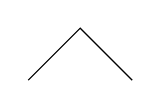
\begin{tikzpicture}[scale=\sc]
\draw  (0,0) -- (3,3) -- (6,0);
\end{tikzpicture}
% \begin{tikzpicture}[scale=\sc]
% \draw  (0,0) -- (3,3);
% \draw  (2,0) -- (5,3);
% \end{tikzpicture}
\quad

\begin{tikzpicture}[scale=\sc]
\draw  (0,0) -- (3,3);
\draw  (3,0) -- (0,3);
\end{tikzpicture}
\\
    \hline
\centering \begin{tikzpicture}[scale=\sc]
\draw  (0,0) -- (3,3);
\end{tikzpicture}
& \centering \parbox[c][\h cm][c]{0.01cm}{  } um terço  &
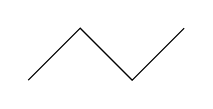
\begin{tikzpicture}[scale=\sc]
\draw  (0,0) -- (3,3) -- (6,0) -- (9,3);
\end{tikzpicture}
% \begin{tikzpicture}[scale=\sc]
% \draw  (0,0) -- (3,3);
% \draw  (2,0) -- (5,3);
% \draw  (4,0) -- (7,3);
% \end{tikzpicture}
 \quad

\begin{tikzpicture}[scale=\sc]
\draw  (0,0) -- (3,3);
\draw  (4,0) -- (1,3);
\draw  (2,0) -- (5,3);
\end{tikzpicture}
\\
    \hline
\centering \begin{tikzpicture}[scale=\sc]
\draw  (0,0) -- (3,3);
\end{tikzpicture}
& \centering \parbox[c][\h cm][c]{0.01cm}{  } um quarto  &
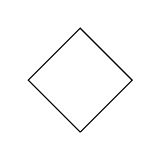
\begin{tikzpicture}[scale=\sc]
\draw  (0,0) -- (3,3) -- (0,6) -- (-3,3) -- (0,0);
\end{tikzpicture}
% \begin{tikzpicture}[scale=\sc]
% \draw  (0,0) -- (3,3);
% \draw  (2,0) -- (5,3);
% \draw  (4,0) -- (7,3);
% \draw  (6,0) -- (9,3);
% \end{tikzpicture}
\quad

\begin{tikzpicture}[scale=\sc]
\draw  (0,0) -- (3,3);
\draw  (4,0) -- (1,3);
\draw  (2,0) -- (5,3);
\draw (2,0) -- (-1,3);
\end{tikzpicture}
\\
\hline
\centering \begin{tikzpicture}[scale=\sc]
\draw [fill=common, fill opacity=.3] (90:2) -- (210:2) -- (330:2) -- cycle;
\end{tikzpicture}  
& \centering \parbox[c][\h cm][c]{0.01cm}{  } metade 
&
\begin{tikzpicture}[scale=\sc]
\draw [fill=common, fill opacity=.3] (90:2) -- (210:2) -- (330:2) -- cycle;
\draw [fill=common, fill opacity=.3, shift={(2*1.732,0)}] (90:2) -- (210:2) -- (330:2) -- cycle;
\end{tikzpicture}
\quad
\begin{tikzpicture}[scale=\sc]
\draw [fill=common, fill opacity=.3] (90:2) -- (210:2) -- (330:2) -- cycle;
\draw [fill=common, fill opacity=.3, rotate around={60:(90:2)}] (90:2) -- (210:2) -- (330:2) -- cycle;
\end{tikzpicture}
\\
    \hline
\centering \begin{tikzpicture}[scale=\sc]
\draw [fill=common, fill opacity=.3] (90:2) -- (210:2) -- (330:2) -- cycle;
\end{tikzpicture}  
& \centering \parbox[c][\h cm][c]{0.01cm}{  } um terço  
&
\begin{tikzpicture}[scale=\sc]
\draw [fill=common, fill opacity=.3] (90:2) -- (210:2) -- (330:2) -- cycle;
\draw [fill=common, fill opacity=.3, shift={(2*1.732,0)}] (90:2) -- (210:2) -- (330:2) -- cycle;
\draw [fill=common, fill opacity=.3, shift={(4*1.732,0)}] (90:2) -- (210:2) -- (330:2) -- cycle;
\end{tikzpicture}
\quad
\begin{tikzpicture}[scale=\sc]
\draw [fill=common, fill opacity=.3] (90:2) -- (210:2) -- (330:2) -- cycle;
\draw [fill=common, fill opacity=.3, shift={(2*1.732,0)}] (90:2) -- (210:2) -- (330:2) -- cycle;
\draw [fill=common, fill opacity=.3, rotate around={120:(330:2)}] (90:2) -- (210:2) -- (330:2) -- cycle;
\end{tikzpicture}
 \quad
\begin{tikzpicture}[scale=\sc]
\draw [fill=common, fill opacity=.3] (90:2) -- (210:2) -- (330:2) -- cycle;
\draw [fill=common, fill opacity=.3, rotate around={60:(90:2)}] (90:2) -- (210:2) -- (330:2) -- cycle;
\draw [fill=common, fill opacity=.3, shift={(2*1.732,0)}] (90:2) -- (210:2) -- (330:2) -- cycle;
\end{tikzpicture}
\\
    \hline
\centering \begin{tikzpicture}[scale=\sc]
\draw [fill=common, fill opacity=.3] (90:2) -- (210:2) -- (330:2) -- cycle;
\end{tikzpicture}  

& \centering \parbox[c][\h cm][c]{0.01cm}{  } um quarto


&
\begin{tikzpicture}[scale=\sc]
\draw [fill=common, fill opacity=.3] (90:2) -- (210:2) -- (330:2) -- cycle;
\draw [fill=common, fill opacity=.3, shift={(2*1.732,0)}] (90:2) -- (210:2) -- (330:2) -- cycle;
\draw [fill=common, fill opacity=.3, shift={(4*1.732,0)}] (90:2) -- (210:2) -- (330:2) -- cycle;
\draw [fill=common, fill opacity=.3, shift={(6*1.732,0)}] (90:2) -- (210:2) -- (330:2) -- cycle;
\end{tikzpicture}
\quad
\begin{tikzpicture}[scale=\sc]
\draw [fill=common, fill opacity=.3] (90:2) -- (210:2) -- (330:2) -- cycle;
\draw [fill=common, fill opacity=.3, rotate around={60:(90:2)}] (90:2) -- (210:2) -- (330:2) -- cycle;
\draw [fill=common, fill opacity=.3, shift={(1.732,3)}] (90:2) -- (210:2) -- (330:2) -- cycle;
\draw [fill=common, fill opacity=.3, shift={(1.732,3)}, rotate around={60:(90:2)}] (90:2) -- (210:2) -- (330:2) -- cycle;
\end{tikzpicture}
\quad
\begin{tikzpicture}[scale=\sc]
\draw [fill=common, fill opacity=.3] (90:2) -- (210:2) -- (330:2) -- cycle;
\draw [fill=common, fill opacity=.3, rotate around={60:(90:2)}] (90:2) -- (210:2) -- (330:2) -- cycle;
\draw [fill=common, fill opacity=.3, rotate around={120:(90:2)}] (90:2) -- (210:2) -- (330:2) -- cycle;
\draw [fill=common, fill opacity=.3, shift={(2*1.732,0)}] (90:2) -- (210:2) -- (330:2) -- cycle;
\end{tikzpicture}
\\
\hline
\end{longtable}
\end{center}
\end{solucao}


\begin{multicols}{2}

  \begin{objetivos}{}{}
\begin{itemize} %s
    \item       Representar uma fração unitária a partir de uma unidade dada.
    \item       Reconhecer (e obter) um quarto como a metade da metade e um oitavo como a metade de um quarto.
    \item       Comparar as frações unitárias metade, um quarto e um oitavo de um mesmo quadrado.
\end{itemize} %s
\end{objetivos}

\begin{orientacoes}
  \begin{itemize} %s
    \item       Esta é uma atividade que o aluno pode fazer individualmente.
    \item       Não se espera que, nesta atividade, os alunos usem a medida para fazer a equipartição de maneira mais precisa. O objetivo é fazer a equipartição livremente e de forma coerente. Assim, por exemplo, podem ser aceitas como respostas:
\end{itemize} %s
\begin{center}
\begin{tikzpicture}[scale=.7]
 \draw[fill=common, fill opacity=.3] (0,0) rectangle (3,3);
 \draw[decorate, decoration={snake, amplitude= .2 mm}] (1.5,0) -- (1.5,3);
\end{tikzpicture}
e
\begin{tikzpicture}[scale=.7]
 \draw[fill=common, fill opacity=.3] (0,0) rectangle (3,3);
 \draw[decorate, decoration={snake, amplitude= .2 mm}] (0,0) -- (3,3);
\end{tikzpicture}
\end{center}
  Já as representações a seguir sugerem que os alunos precisam revisar os conceitos exigidos para a solução da atividade:
\begin{center}
  \begin{tikzpicture}[scale=.7]
 \draw[fill=common, fill opacity=.3] (0,0) rectangle (3,3);
 \draw[decorate, decoration={snake, amplitude= .2 mm}] (2.3,0) -- (2.3,3);
\end{tikzpicture}
\end{center}
\begin{itemize} %s
    \item       A representação da unidade se dá de forma genérica por um quadrado.
    \item       Espera-se que os alunos reconheçam que, para obter um quarto da unidade, basta tomar a metade da metade. E que, para determinar um oitavo, pode-se dividir um quarto ao meio.
    \item       Recomenda-se que os alunos tenham em mãos três quadrados de papel iguais e que sejam orientados a fazer uso de dobradura para identificar as frações pedidas. Assim, por exemplo, a fração um quarto pode ser obtida por duas dobras do papel.
    \item Discuta com os estudantes que, quanto maior o número de partes iguais em que se particiona o quadrado, menor fica cada uma das partes.
    \item Procure apresentar e discutir com a turma mais do que uma solução para cada item.
    \item \textbf{As diferentes soluções apresentadas pelos alunos podem enriquecer a discussão}. A comparação entre, por exemplo, a metade do quadrado proveniente da dobradura pela diagonal e o quarto do quadrado proveniente da dobradura a partir de linhas paralelas aos lados (como um sinal de ``$+$'') pode não ser tão natural. Dificuldade semelhante pode ser observada na comparação entre esse mesmo quarto do quadrado e o oitavo do quadrado proveniente de uma sequência de dobraduras paralelas a um dos lados, determinando ``faixas paralelas''. Nesses casos, para executar a comparação, é necessário que os alunos reconheçam partes de formatos diferentes que correspondem a uma mesma fração do quadrado como iguais em quantidade (no caso, área). Assim, a comparação entre a metade do quadrado, obtida pela dobradura na diagonal, e o quarto do quadrado, obtido pela dobradura ``em sinal de $+$'', pode ser amparada pelo reconhecimento de que a metade em questão é igual em quantidade (área) à metade do quadrado obtida por uma única dobra paralela a um dos lados, que é o dobro do quarto do quadrado.

\begin{center}
  \begin{tikzpicture}[scale=.5]
         \draw[fill=common, fill opacity=.3] (0,0) rectangle (2,2);
         \draw[fill=attention] (0,1) rectangle (2,2);
        \end{tikzpicture}\quad\quad
        \begin{tikzpicture}[scale=.5]
         \draw[fill=common, fill opacity=.3] (0,0) rectangle (2,2);
         \draw[fill=attention] (0,0) -- (2,2) -- (0,2)--cycle;
        \end{tikzpicture}
\end{center}

\item Nossa experiência na implementação desta atividade com estudantes do $6^\circ$ ano mostrou que após os alunos entenderem que se espera mesma quantidade e não mesmo formato, passaram a se divertir indo ao quadro para exibir equipartições diferentes daquelas já exibidas pelos colegas.
\end{itemize} %s
\end{orientacoes}

\begin{solucao}{}{}
  Algumas soluções possíveis, convencionais e outras menos convencionais são:

        \begin{enumerate}[a)]
         \item Metade:   \newline
        \begin{tikzpicture}[scale=.8]
         \draw[fill=common, fill opacity=.3] (0,0) rectangle (2,2);
         \draw[fill=attention] (0,1) rectangle (2,2);
        \end{tikzpicture}
        \begin{tikzpicture}[scale=.8]
         \draw[fill=common, fill opacity=.3] (0,0) rectangle (2,2);
         \draw[fill=attention] (0,0) -- (2,2) -- (0,2)--cycle;
        \end{tikzpicture}
        \begin{tikzpicture}[scale=.8]
         \draw[fill=common, fill opacity=.3] (0,0) rectangle (2,2);
         \draw[fill=attention] (0,2) -- (2,2) -- (1,1)--cycle;
         \draw[fill=attention] (0,0) -- (2,0) -- (1,1)--cycle;
        \end{tikzpicture}
        \begin{tikzpicture}[scale=.8]
         \draw[fill=common, fill opacity=.3] (0,0) rectangle (2,2);
         \draw[fill=attention] (0,1) rectangle (1,2);
         \draw[fill=attention] (1,0) rectangle (2,1);
        \end{tikzpicture}
       \item Um quarto:  \newline
       \begin{tikzpicture}[scale=.8]
         \draw[fill=common, fill opacity=.3] (0,0) rectangle (2,2);
         \draw[fill=attention] (0,0) rectangle (.5,2);
         \foreach \x in {1,1.5} \draw (\x,0) -- (\x,2);
       \end{tikzpicture}
       \begin{tikzpicture}[scale=.8]
         \draw[fill=common, fill opacity=.3] (0,0) rectangle (2,2);
         \draw[fill=attention] (0,1) rectangle (1,2);
         \draw (1,0) -- (1,1);
         \draw (1,1)-- (2,1);
        \end{tikzpicture}
        \begin{tikzpicture}[scale=.8]
         \draw[fill=common, fill opacity=.3] (0,0) rectangle (2,2);
         \draw[fill=attention] (0,0) -- (1,1) -- (0,2)--cycle;
         \draw (1,1) -- (2,2);
         \draw (1,1) -- (2,0);
        \end{tikzpicture}
        \begin{tikzpicture}[scale=.8]
         \draw[fill=common, fill opacity=.3] (0,0) rectangle (2,2);
         \draw[fill=attention] (2,2) -- (1,2) -- (1,1)--cycle;
         \draw[fill=attention] (0,0) -- (1,0) -- (1,1)--cycle;
         \draw (0,2) -- (2,0);
        \end{tikzpicture}
       \item  Um oitavo:  \newline
       \begin{tikzpicture}[scale=.8]
         \draw[fill=common, fill opacity=.3] (0,0) rectangle (2,2);
         \draw[fill=attention] (0,0) rectangle (.25,2);
         \foreach \x in {.5,.75,...,1.75} \draw (\x,0) -- (\x, 2);
       \end{tikzpicture}
       \begin{tikzpicture}[scale=.8]
         \draw[fill=common, fill opacity=.3] (0,0) rectangle (2,2);
         \draw[fill=attention] (0,1) rectangle (.5,2);
         \draw (0,1)--(2,1);
         \foreach \x in {.5,1,...,1.5} \draw (\x,0) -- (\x,2);
        \end{tikzpicture}
        \begin{tikzpicture}[scale=.8]
         \draw[fill=common, fill opacity=.3] (0,0) rectangle (2,2);
         \draw[fill=attention] (0,1) -- (1,1) -- (0,2)--cycle;
         \draw (0,0) -- (1,1);
        \end{tikzpicture}
        \begin{tikzpicture}[scale=.8]
         \draw[fill=common, fill opacity=.3] (0,0) rectangle (2,2);
         \draw[fill=attention] (2,2) -- (1,2) -- (1,1)--cycle;
         \draw (1,1) -- (1,0);
         \draw (0,0) -- (1,1);
         \end{tikzpicture}
       \item  Dentre as opções apresentadas, a maior fração do quadrado é metade.
        \end{enumerate}
\end{solucao}

\begin{objetivos}{}{}
\begin{itemize} %s
    \item       Representar uma fração unitária (no caso, um meio ou metade) a partir de uma unidade não usual dada.
    \item       Estabelecer representações diferentes para a mesma fração unitária de uma mesma unidade.
\end{itemize} %s
 \end{objetivos}

\begin{orientacoes}
\begin{itemize} %s
   \item Esta é uma atividade que o aluno pode fazer individualmente. Mas caso os estudantes tenham dificuldades em encontrar três representações distintas, sugere-se que sejam socializadas suas respostas, quando provavelmente aparecerão mais do que três soluções distintas.
   \item Observe que a representação da unidade se dá de forma genérica, ainda em modelo contínuo, por uma figura não tradicional como retângulos e círculos, que é determinada pela justaposição de dois hexágonos regulares.
   \item       Como na atividade anterior, não se espera que, nesta atividade, o aluno use a medida para fazer a equipartição de maneira mais precisa. O objetivo é que o aluno faça a equipartição livremente e de forma coerente,  mesmo porque aqui não se recomenda o uso de material concreto para a realização da atividade. É esperado que o material concreto utilizado como apoio para as atividades anteriores já seja suficiente para que o estudante abstraia a ideia de equipartição e faça uso de sua imaginação apenas.
   \item Procure apresentar e discutir com a turma mais do que uma solução para cada item.
\end{itemize} %s
\end{orientacoes}

\begin{solucao}{}{}
Algumas das respostas possíveis para este problema são:
\begin{center}
\begin{tikzpicture}[scale=.4]
\draw[fill=attention] (3.,5.) -- (3.,3.) -- (4.7,2.) -- (6.46,3.) -- (6.46,5.) -- (4.73,6.) -- cycle;
\draw[fill=common, fill opacity=.3] (6.46,5.) -- (6.46,3.) -- (8.2,2.) -- (9.9,3.) -- (9.9,5.) -- (8.2,6.) -- cycle;
\end{tikzpicture}\hspace{.2cm}
\begin{tikzpicture}[scale=.4]
\draw[fill=common, fill opacity=.3] (3.,5.) -- (3.,3.) -- (4.7,2.) -- (6.46,3.) -- (6.46,5.) -- (4.73,6.) -- cycle;
\draw[fill=common, fill opacity=.3] (6.46,5.) -- (6.46,3.) -- (8.2,2.) -- (9.9,3.) -- (9.9,5.) -- (8.2,6.) -- cycle;
\draw[fill=attention] (4.732050807568877,6.) -- (3.,5.) -- (3.,3.) -- (4.732050807568877,2.) -- cycle;
\draw[fill=attention] (8.2,6.) -- (8.2,2.) -- (9.9,3.) -- (9.9,5.) -- cycle;
\end{tikzpicture}

\begin{tikzpicture}[scale=.4]
\draw[fill=common, fill opacity=.3] (3.,5.) -- (3.,3.) -- (4.7,2.) -- (6.46,3.) -- (6.46,5.) -- (4.73,6.) -- cycle;
\draw[fill=common, fill opacity=.3] (6.46,5.) -- (6.46,3.) -- (8.2,2.) -- (9.9,3.) -- (9.9,5.) -- (8.2,6.) -- cycle;
\draw[fill=attention] (3.,4.) -- (3.,3.) -- (4.732050807568877,2.) -- (6.464101615137757,3.) -- (8.196152422706634,2.) -- (9.928203230275509,3.) -- (9.928203230275509,4.) -- cycle;
\end{tikzpicture}\hspace{.2cm}
\begin{tikzpicture}[scale=.4]
\draw[fill=common, fill opacity=.3] (3.,5.) -- (3.,3.) -- (4.7,2.) -- (6.46,3.) -- (6.46,5.) -- (4.73,6.) -- cycle;
\draw[fill=common, fill opacity=.3] (6.46,5.) -- (6.46,3.) -- (8.2,2.) -- (9.9,3.) -- (9.9,5.) -- (8.2,6.) -- cycle;
\draw[fill=attention] (3,5) -- (3.,3.) -- (4.73,2.) -- (6.46,3.) -- (8.2,2.) -- (9.9,3.) -- cycle;
\end{tikzpicture}
\end{center}
\end{solucao}

\begin{objetivos}{}{}
\begin{itemize} %s
    \item       Reconhecer a metade de uma unidade pela reunião de partes menores e em partições diversas.
    \item       Estabelecer representações diferentes para a mesma fração unitária para uma mesma unidade.
\end{itemize} %s
\end{objetivos}

\begin{orientacoes}
  \begin{itemize} %s
  \item       Esta é uma atividade que o aluno pode fazer individualmente.
  \item       Cada aluno deve receber as imagens das figuras, disponíveis para reprodução no final do livro para que possa manipular como achar melhor e conduzir a sua decisão.
  \item       Esta atividade pretende levar o aluno a perceber que a metade de uma unidade pode ser considerada e identificada mesmo sem que se tenha uma divisão em duas partes iguais.
  \item       Como nas atividades anteriores, não se espera que o aluno use a medida para confirmar a metade da unidade. O objetivo é que o aluno identifique a representação da metade (ou não) por sobreposição e justaposição das partes, decompondo e recompondo a figura.
  \item       Incentive os alunos a argumentar, justificando a sua decisão. Para isso, podem, por exemplo, se apoiar em dobraduras ou em recortes das partes da figura.
  \item       Procure apresentar e discutir com a turma mais do que uma solução para cada item.
\end{itemize} %s
\end{orientacoes}

\begin{solucao}{}{}
  As figuras que correspondem à metade da unidade são as de números 1, 2, 4, 5, 6, 8, 9, 11 e 12.
\end{solucao}

\begin{objetivos}{}{}
\begin{itemize}
 \item Distinguir e nomear frações unitárias a partir de suas representações em modelos circulares.
\item  Comparar frações unitárias a partir de suas representações em modelos circulares.
\end{itemize}
\end{objetivos}

\begin{orientacoes}
\begin{itemize}
\item    Esta atividade é planejada para ser desenvolvida a partir de material concreto baseado em modelos circulares. Mais especificamente com um material conhecido como ``Círculos de Frações''. Para aplicá-la, é necessário reproduzir esse material, que está disponível nas páginas para reprodução.
\item Sendo um material concreto, os círculos de frações têm o papel de auxiliar na visualização da representação das frações, mais especificamente, das frações unitárias.
\item Recomenda-se que esta atividade seja desenvolvida em grupos de 3 a 5 alunos. No entanto, cada aluno deve ter o seu próprio material (Círculos de Frações) para realizar a atividade.
\item Durante a discussão, os alunos devem ser estimulados a explicar as suas escolhas. O uso de cores vai fazer parte da comunicação, no entanto a justificativa e raciocínio devem estar apoiados no conceito de fração.
 \item Na versão utilizada nesta atividade, o círculo corresponde à unidade, ou seja, ao 1 e os setores circulares, diferenciados por cores, correspondem às frações unitárias um meio, um terço, um quarto, um sexto, um sétimo, um oitavo, um nono e um décimo.
    \item Refira-se ao círculo na cor preta como círculo ou unidade, e não como todo ou inteiro. Refira-se a cada setor circular como fração do círculo, parte do círculo ou, simplesmente, peça da cor x.
    \item Antes de solicitar aos alunos que realizem a atividade, explore o material ressaltando especialmente o fato de que, reunidas, as peças de uma mesma cor determinam um círculo congruente ao preto.
    \item Ainda antes de solicitar aos alunos que realizem a atividade, explore também o material com perguntas dirigidas a toda a turma como as seguintes: ``Quantas peças azuis cobrem o círculo preto?'' ou ``Quantas peças verdes cobrem o círculo preto?'', sugerindo que as peças coloridas podem ser consideradas frações do círculo preto.
    \item Faça uso do material concreto para ilustrar e explicar a resposta de cada item e incentive os seus alunos a fazerem o mesmo.
    \item Espera-se que a explicação para as respostas, nos oito primeiros itens desta questão, seja a partir da contagem dos setores circulares correspondentes às frações envolvidas. Assim, por exemplo, a resposta do item b) pode ser justificada pelo fato de que são necessários 4 partes de círculo na cor vermelha para compor um círculo preto.
    \item Já para os cinco itens que tratam da comparação, espera-se que os alunos identifiquem os setores que representam as frações envolvidas e procedam a comparação pela sobreposição das peças correspondentes. Assim, por exemplo, a resposta do item l) pode ser justificada pela sobreposição das peças das cores verde e amarelo.
    \item Aproveite a correção desses últimos itens para explorar, a partir dos Círculos de Frações, a relação entre a quantidade de peças de cada cor e o tamanho das peças, ou seja, a relação inversa entre a quantidade de partes em que círculo (unidade) está dividido e o tamanho de cada parte.
    \item Os Círculos de Frações podem ser utilizados para trabalhar outros conceitos e assuntos além de frações unitárias, tais como: frações em geral, comparação de frações e operações com frações (adição e subtração). 
    \end{itemize}
\end{orientacoes}
  \end{multicols}


\begin{solucao}{}{}
  % Faltam as justificativas.
\begin{enumerate}[a)]
 \item Uma peça da cor AZUL é igual a um terço do círculo preto.
 \item    Uma peça da cor VERMELHA é igual a um quarto do círculo preto.
 \item    Uma peça da cor AMARELA é igual a um sétimo do círculo preto.
 \item    Uma peça da cor LARANJA é igual a um nono do círculo preto.
 \item    Uma peça da cor roxa é igual a UM SEXTO do círculo preto.
 \item    Uma peça da cor cinza é igual a UM OITAVO do círculo preto.
 \item    Uma peça da cor branca é igual a UM DÉCIMO do círculo preto.
 \item    Uma peça da cor rosa é igual à METADE do círculo preto.
 \item    Um terço do círculo preto é maior do que um sétimo do círculo preto.
 \item    Um nono do círculo preto é menor do que um quarto do círculo preto.
 \item    Um sétimo do círculo preto é menor do que um quinto do círculo preto.
 \item    Um quarto do círculo preto é maior do que um oitavo do círculo preto.
 \item    Um sexto do círculo preto é maior do que um sétimo do círculo preto
\end{enumerate}

\end{solucao}

\begin{objetivos}{}{}
  \begin{itemize} %s
    \item Conhecer e compreender as expressões correspondentes às frações unitárias com denominadores de 5 a 10.
    \item Comparar frações da unidade por meio da representação visual de frações do círculo.
    \item Reconhecer a relação inversa entre o número de partes e o tamanho de cada parte.
\end{itemize} %s
\end{objetivos}

\begin{orientacoes}
\begin{itemize} %s
    \item       Esta atividade pode ser resolvida individualmente, mas é essencial que seja discutida com toda a turma.
    \item       É provável que nem todos os alunos conheçam ou intuam as expressões correspondentes às frações propostas. Nesse caso, cabe ao professor apresentá-las e diferenciá-las.
    \item       Aproveite esta atividade para revisar e discutir o vocabulário que é objetivo nesta seção:       {\it unidade,}             {\it metade,}             {\it um meio,}             {\it um terço,}             {\it terça parte,}             {\it um quarto,}             {\it quarta parte,}             {\it um quinto,}             {\it quinta parte,}             {\it um sexto,}             {\it sexta parte,}             {\it um sétimo,}             {\it sétima parte,}             {\it um oitavo,}             {\it oitava parte,}             {\it um nono,}             {\it nona parte,}             {\it um décimo}       e       {\it décima parte}      .
\end{itemize} %s
\end{orientacoes}

\newpage
\begin{solucao}{}{}
\begin{enumerate}[a),wide,labelindent=0pt] %s
    \item       A correspondência adequada é:
\begin{enumerate} [\;\; I), labelindent=0pt] %d
        \item           A esta afirmação corresponde à figura G).
        \item           A esta afirmação corresponde à figura D).
        \item           A esta afirmação corresponde à figura I).
        \item           A esta afirmação corresponde à figura B).
        \item           A esta afirmação corresponde à figura A).
        \item           A esta afirmação corresponde à figura F).
\end{enumerate} %d

    \item       As frações um sétimo, um oitavo, um nono e um décimo do círculo são menores que um sexto do círculo. Qualquer uma delas está correta. Portanto qualquer uma delas serve como resposta.
    \item       As frações um meio, um terço, um quarto, um quinto, um sexto, um sétimo e um oitavo do círculo são maiores que um nono do círculo. Qualquer uma delas está correta.
    \item       As frações um sétimo e um oitavo do círculo são menores que um sexto e maiores que um nono do círculo.
\end{enumerate} %s
\end{solucao}

\pagebreak
\begin{objetivos}{}{}
\begin{itemize} %s
    \item Reconhecer e diferenciar a representação das frações ``um meio'', ``um quarto'' e       ``um décimo'' em modelos diversos, baseados  ou não em equipartição.
\end{itemize} %s
\end{objetivos}

\begin{orientacoes}
\begin{itemize} %s
\item       Esta é uma atividade que o aluno pode fazer individualmente.
\item Esta atividade pode ser desenvolvida com o uso do material para reprodução disponível no final do livro caso se entenda que seus estudantes ainda precisam deste recurso.
\item Como nas atividades anteriores, não se espera que os alunos usem a medida para confirmar a metade. O objetivo é que identifiquem a representação da metade (ou não) por sobreposição e justaposição dessas partes, decompondo e recompondo a figura.
\item No item m), pretende-se que o estudante considere o quadrado maior como unidade e perceba que a parte em vermelho corresponde à metade desse quadrado. Isso pode ser feito observando que todos os quadradinhos vermelhos podem ser agrupados para formar a metade superior do quadrado maior e os azuis agrupados para formar a parte de baixo, por exemplo.
\begin{center}
  \begin{tikzpicture}[scale=.5]
\draw[fill=common, fill opacity=.3] (0,0) rectangle (4,4);
 \filldraw[fill=attention, draw=black] (1,0) rectangle (2,1);
 \filldraw[fill=attention, draw=black] (3,0) rectangle (4,1);
 \filldraw[fill=attention, draw=black] (0,1) rectangle (1,2);
 \filldraw[fill=attention, draw=black] (2,1) rectangle (3,2);
 \filldraw[fill=attention, draw=black] (1,2) rectangle (2,3);
 \filldraw[fill=attention, draw=black] (3,2) rectangle (4,3);
 \filldraw[fill=attention, draw=black] (0,3) rectangle (1,4);
 \filldraw[fill=attention, draw=black] (2,3) rectangle (3,4);
\end{tikzpicture}
\quad
\begin{tikzpicture}[scale=.5]
  \draw[fill=common, fill opacity=.3] (0,0) rectangle (4,4);
  \filldraw[fill=attention, draw=black] (0,2) rectangle (4,4);
  \draw (0,0) grid (4,4);
\end{tikzpicture}
\end{center}

Neste item m), é prematuro e, portanto, inadequado usar o argumento de que a fração é um meio argumentando que dos 16 quadradinhos, existem 8 pintados de vermelho. Isso porque, nessa linha de raciocínio, a unidade seria o quadradinho e não o quadrado maior e, consequentemente, não se estaria fazendo uma divisão de uma unidade mas, sim, uma contagem em um modelo discreto de frações, abordagem essa que escolhemos evitar nesse momento.   


\item Incentive os alunos a argumentar, justificando a sua decisão. Para isso, podem, por exemplo, se apoiar em dobraduras ou no recorte das partes da figura.
\item Procure apresentar e discutir com a turma mais do que uma solução para cada item.
\end{itemize} %s
\end{orientacoes}

\begin{solucao}{}{}
  \begin{tabular}{lll}
a) um meio,&  b) um décimo,& c) um quarto,\\
d) um quarto,& e) um quarto,& f) um meio,\\
g) um quarto,& h) um décimo,& i) um quarto,\\
j) um décimo,& l) um quarto,& m) um meio
\end{tabular}
\end{solucao}



%%% Local Variables: 
%%% mode: latex
%%% TeX-master: "livro_professor_completo.tex"
%%% End: 